
\section{Results \& Discussion}

\subsection{Binding energy}
 \begin{table}[ht]
     \caption{Binding energy (meV) of a hydrogen atom chemisorbed on graphene calculated with various DFT functionals and with DMC.}
    \centering
    \begin{tabular}{lr}%\hline%\toprule
    Method & Binding energy\\\hline \\\\[-2em]%
    \multicolumn{2}{c}{\bfseries This Work} \\
    PBE \tnote{1} & -821\\ %-820.5815227
    PBE\tnote{2} & -871\\ 
    PBE0\tnote{2}& -851 (-800)\\ 
    HSE\tnote{2}& -794 (-743)\\ 
    DMC  & -691 $\pm$ 19 \\ \hline \\\\[-2em]%-690.8154569 $\pm$ 18.61340357
    \multicolumn{2}{c}{\bfseries Previous Work}\\
    PW91  &  -810 to -830\cite{10.1063/1.3187941}, -870\cite{10.1103/PhysRevLett.93.187202}\\
    PBE  & -790\cite{10.1103/PhysRevB.78.041402}, -840\cite{10.1063/1.3072333}, -980\cite{10.1088/0957-4484/19/15/155708}\\
     \hline%\bottomrule
    \end{tabular}
\label{tab:summary_energetics}
\begin{tablenotes}
\item[1] Calculation was done in the plane wave basis.
\item[2] Calculation was done in the Gaussian basis set with corrections for BSSE. Values in parentheses include a correction for the basis set incompleteness as described in the text.
\end{tablenotes}

 \end{table}
 

Table~\ref{tab:summary_energetics} contains a summary of the binding energies of a hydrogen atom chemisorbed on graphene from this work and selected values from previous publications using the PW91 and PBE functionals.
These literature values range from -790 to -980 meV.
This wide spread of binding energies is caused by (1) the use in some studies of small supercells for which there are sizable interactions between the CH groups in adjacent cells, and (2) the use in some studies of small atom-centered basis sets without corrections for BSSE.
Our calculations with the PBE functional in conjunction with a plane wave basis set give a binding energy of -821 meV. 
This should be contrasted with our -691 $\pm$ 19 meV DMC result.
There are several possible sources for the difference between the PBE and DMC values of the binding energy. 
These include errors in the DFT calculations due to self interaction and planar graphene having more multiconfigurational character than H/graphene, with this being better described with DMC than with PBE.
We note that the inclusion of the D3 dispersion correction with the PBE functional only changes the magnitude of the binding energy by 0.03 eV.

The PBE binding energy is 51 meV lower in magnitude in the plane wave than in the GTO basis set when the same $k$-point grid is used, and this value is used as a correction for the basis set incompleteness error for the results with other functionals in Table~\ref{tab:summary_energetics}.
The calculations in the GTO basis set give a slightly smaller in magnitude binding energy with PBE0 than with PBE.
However, with HSE, we obtain a binding energy 77 meV smaller in magnitude than the PBE result.
Applying the correction for the basis set incompleteness error, we obtain -800 meV for the PBE0 binding energy and -743 meV for the HSE binding energy, with the latter being in reasonable agreement with the DMC result of -691 meV.
Although the 130 meV difference between the plane-wave PBE and DMC values of the binding energy may appear to be small, this energy difference, of that magnitude is consistent with an order of magnitude change in the hydrogen evolution current at room temperature on graphene electrodes.\cite{10.1021/acsami.1c21821}


 
In order to better understand the origin of the difference in the PBE and HSE H-atom adsorption energies, we also carried out non-self-consistent calculations, using PBE densities to evaluate the HSE energies.  These calculations gave a binding energy only 21 meV smaller in magnitude than obtained from the self-consistent HSE calculations.  This demonstrates that the functional is more important than the density in establishing the binding energy. Detailed information can be found in Table S4 of the Supplementary Material.
 
Detailed results of the DMC calculations can be found in Tables S5-S7 in the Supplementary Material.

\subsection{Binding density}

\begin{figure*}
    \centering
    \includegraphics[width=\textwidth,keepaspectratio]{Images/chapter4/hgraphene_minus_distgraphene_minusH_montage_labelled_lowres.png}
    \caption{Change of the electron density due to the adsorption of the H atom to the distorted graphene sheet (Eq.~\ref{eq:bindingdensity}). $\rho_b$ from PBE calculations is shown from an oblique angle (A) and aligned along the $c$ axis (B). $\rho_b$ from DMC calculations (C) and (D) is shown from the same perspectives. Gold and blue represent a gain and loss of electron density, respectively. Note that there is a region of increased charge density at the C-H bond that is enveloped by a region of loss in the charge density. The binding density was visualized using an isovalue of 2.8$\times10^{-5}$ for DMC and 3.9$\times10^{-5}$ for PBE, in both cases capturing 95\% of the differential charge density.}
    \label{fig:densdiff}
\end{figure*}
It is instructive to examine the change in the electron density associated with the binding of the H atom to the distorted graphene as determined from the PBE and DMC calculations.
The density change is given by
\begin{equation}
\rho_b=\rho_{dgr+H}-(\rho_{dgr}+\rho_{H}),
\label{eq:bindingdensity}
\end{equation}
where $\rho_{H}$ is the charge density of the hydrogen atom, and $\rho_{dgr+H}$ and $\rho_{dgr}$ are the charge densities of the distorted graphene sheet with and without hydrogen, respectively. For the QMC density, the density was accumulated during the VMC and DMC calculations, the mixed estimator bias was found to be insignificant, and was thus not corrected.

The $\rho_b$ density differences for both DMC and PBE are shown in Figure \ref{fig:densdiff}. 
The dark blue and gold regions represent a loss and gain of electron density, respectively.
As expected, there is a shift in electron density from the carbon atom participating in the carbon-hydrogen bond as well as to the three adjacent carbon atoms. 
These qualitative changes in the density are consistent with previous theoretical and experimental studies.\cite{10.1063/1.4896611,10.1126/science.aaw6378}
The rehybridization from $sp^2$ to $sp^3$ of the carbon participating in the CH bond and the weakening of the $\pi$ bonds due to the distortion of the graphene lead to the electron density shift.
The change in the charge distribution is similar for PBE and DMC, with the most noticeable difference being a greater increase of density at remote C atoms in the DMC than in the PBE calculations.

\subsection{Charge density differences between DMC and PBE}
In this section, the difference between the DMC and PBE charge densities for distorted graphene with the adsorbed hydrogen atom as well as for pristine planar graphene without the adsorbed hydrogen atom are considered. 
The charge density difference for each system is calculated according to 
\begin{equation}
    \Delta\rho_{system} =\rho_{system}^{DMC}- \rho_{system}^{PBE},
    \label{eq:densdiff}
\end{equation}
where $\rho_{system}^{DMC}$ is the DMC charge density of a given system (either distorted graphene with the adsorbed hydrogen or pristine graphene) and $\rho_{system}^{PBE}$ is the corresponding PBE charge density.
$\Delta\rho_{gr}$ and $\Delta\rho_{dgr+H}$ are reported in Figure~\ref{fig:densdiff_dmcminusdft} along the 110 slice through the unit cell, which captures the carbon-hydrogen bond.
From the top-down perspective in Figure~\ref{fig:cell}, the 110 lattice plane bisects the cell diagonally through the longer of the two diagonals and is indicated by the solid cyan line.
In Figure~\ref{fig:densdiff_dmcminusdft}, blue represents areas where the PBE density is larger, while gold areas represent areas where the DMC density is larger.
The DMC density, in comparison with the PBE density, has greater weight in the bonding region between atoms.
We note that the HSE density displays similar differences as the PBE density. Figure S2 of the Supplementary Material includes a visualization of the DMC-HSE density difference.
This is the case for both the planar graphene without hydrogen and the system with hydrogen chemisorbed to graphene.
Even though there are significant differences between the PBE and DMC densities for both systems, the difference is similar in the two systems, consistent with it not introducing a large error in the PBE value of the binding energy.


\begin{figure}
    \centering
    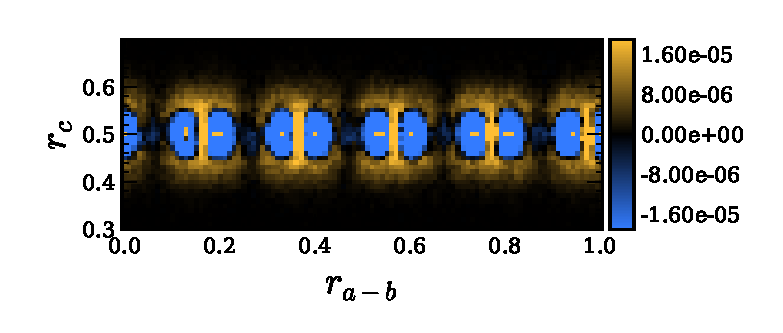
\includegraphics[width=\columnwidth,keepaspectratio]{Images/chapter4/qmc_2d_slice_graphene.eps}
    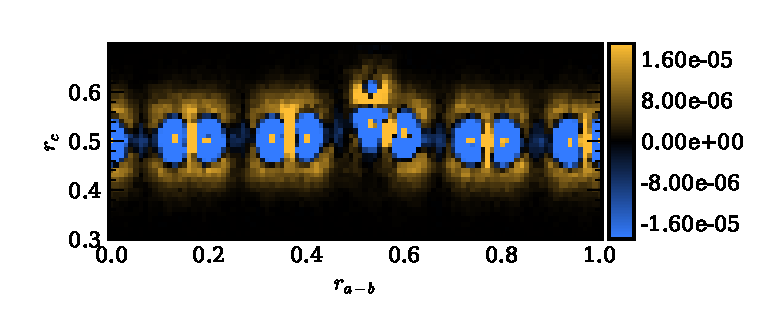
\includegraphics[width=\columnwidth,keepaspectratio]{Images/chapter4/qmc_2d_slice_hgraphene.eps}
    \caption{Visualization of the difference of PBE and DMC densities sliced along the 110 lattice plane of the unit cell for the graphene sheet, $\Delta\rho_{gr}$, (top) and H adsorbed onto graphene, $\Delta\rho_{dgr+H}$, (bottom). The abscissa represents traversing the 110 plane in fractional coordinates, while the ordinate represents traversing the $c$ axis in fractional coordinates. Blue regions represent places where the PBE density is larger, while the gold color represents regions where the DMC density is larger. }
    \label{fig:densdiff_dmcminusdft}
\end{figure}

%%%%%%%%%%%%%%%%%%%%%%%%%%%%%%%%%%%%%%%%%%%%%%%%%%%%%%%%%
